\section{Group in the Filament}
\label{sec:Group}

\begin{figure*}
	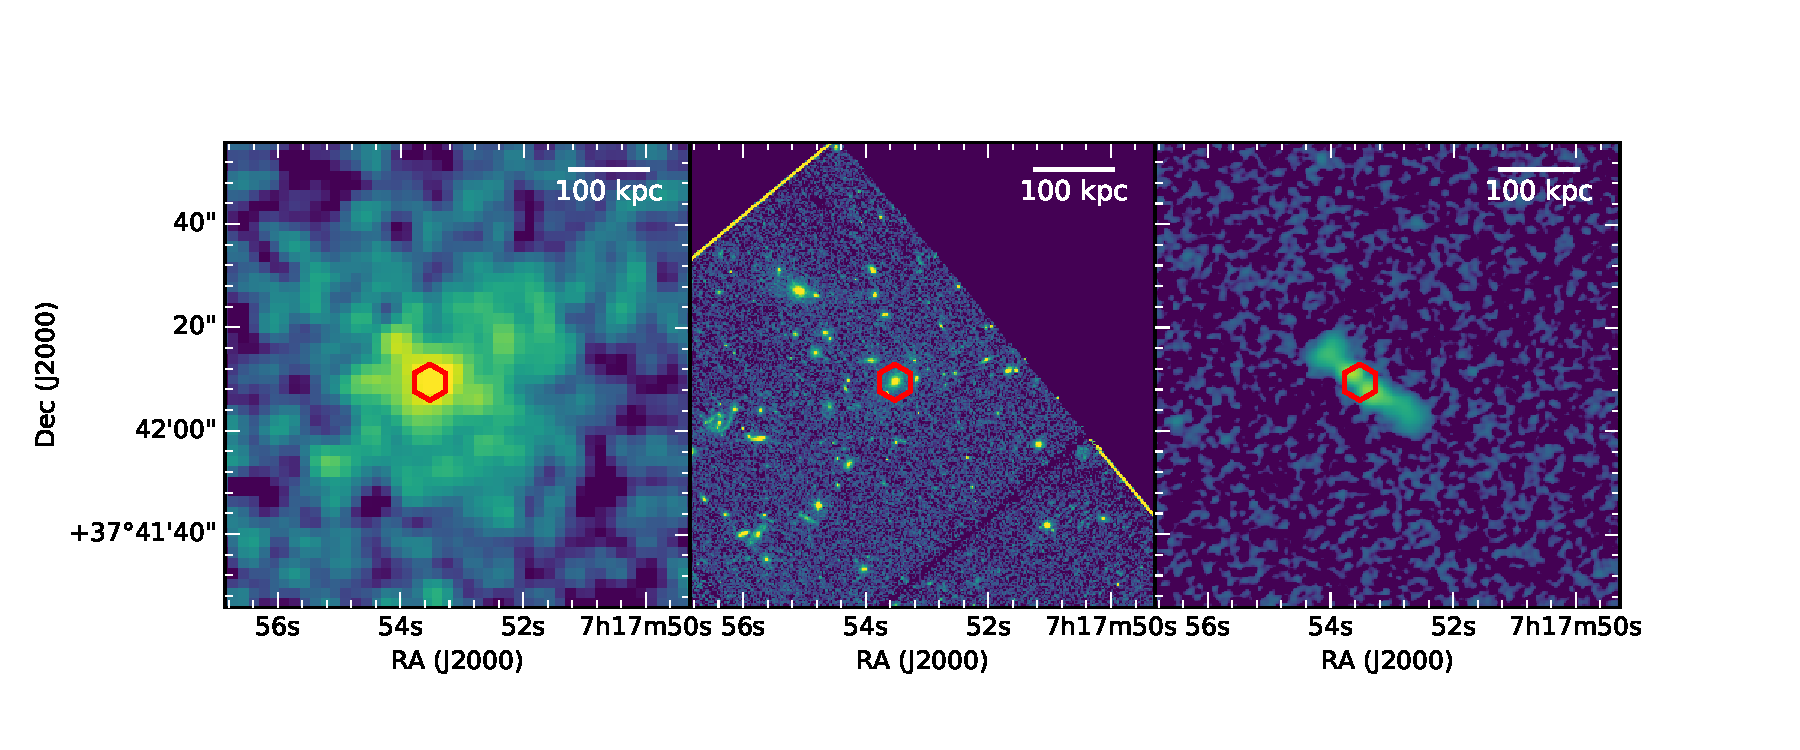
\includegraphics[width=\textwidth]{plots/group_bcg.pdf}
	\caption{$0.5-4$~keV  \chandra\ (left), F606W \emph{HST} (middle; PropID 10084), and $1-2$~GHz L-band A-array \emph{VLA} (right) images of the region occupied by the galaxy group in the filament. The red hexagon marks the position of the group's centrally dominant galaxy (BCG). The size of the radio beam (10.7~kpc~$\times$~9.0 kpc) is shown in the bottom left corner of the radio image. Results from the radio data are described by van Weeren et al., submitted. The position of the BCG coincides with those of the radio AGN and of the X-ray peak.\label{fig:group}}
\end{figure*}

The group of galaxies within the large-scale filament is located in projection a little over 2~Mpc SE of the cluster center, fixed at ${\rm RA} = 07^{\rm h}\, 17^{\rm m}\, 30.025^{\rm s}$, ${\rm Dec} = +37^{\circ}\, 45\arcmin \, 18.58\arcmin\arcmin$ for consistency with \citet{Jauzac2012}. The small size of the group and its large distance from the cluster implies that it is falling for the first time towards MACS~J0717.5+3745, rather than having traversed the cluster from the NW to the SE. This interpretation is also supported by the fact that the position of the X-ray peak is consistent with those of the cD galaxy and of the AGN hosted by the galaxy, as seen in Figure~\ref{fig:group}.

We measured the temperature and the brightness of the group by extracting spectra within $r_{\rm 2500} \approx 300$~kpc \citep{Medezinski2013}. The circular region, shown in Figure~\ref{fig:fil}, had the center fixed at ${\rm RA} = 07^{\rm h}\, 17^{\rm m}\, 53.347^{\rm s}$, ${\rm Dec} = +37^{\circ}\, 42\arcmin \, 09.25\arcmin\arcmin$. We assumed a group metallicity of 0.2 solar \citep[e.g.,][]{Rasmussen2007}. The best-fitting parameters are summarized in Table~\ref{tab:spectra}. The cluster has a $r_{2500}$ temperature of $4.19_{-0.48}^{+0.76}$~keV. The normalization is equivalent to a bolometric luminosity of $(1.2\pm 0.1) \times 10^{44}$~erg~s$^{-1}$. Based on the luminosity-mass scaling relations for galaxy groups \citep[e.g.,][]{Connor2014}, the group's luminosity corresponds to $M_{\rm 2500} \sim 5\times 10^{13}$~M$_\odot$. A consistent mass estimate is obtained from the temperature-mass scaling relations.  Using optical data, \citet{Medezinski2013} determined $M_{\rm 2500} = (7.4\pm 3.0) \times 10^{13}$~M$_\odot$, which is also consistent with our estimate. The group thus sits on the luminosity-mass and temperature-mass relations, which is further indication that no significant stripping by the cluster has occurred yet.
